
\chapter{Python Code}\label{ch:Python Code}

Code goes here

\chapter{Data Description}\label{ch:Data Description}

\begin{figure}[h!]
    \centering
    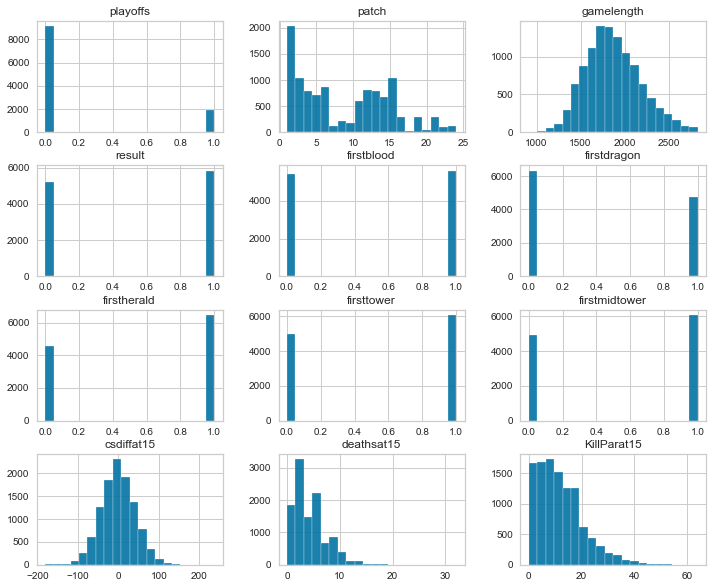
\includegraphics[width=1\textwidth]{figures/DistributionVisualisation}
    \caption{Graphs showing the distribution of data for the dataset}
    \label{fig:DistroVisual}
\end{figure}

\chapter{Feature Correlations}\label{ch:Feature Correlations}

\begin{figure}[h!]
    \centering
    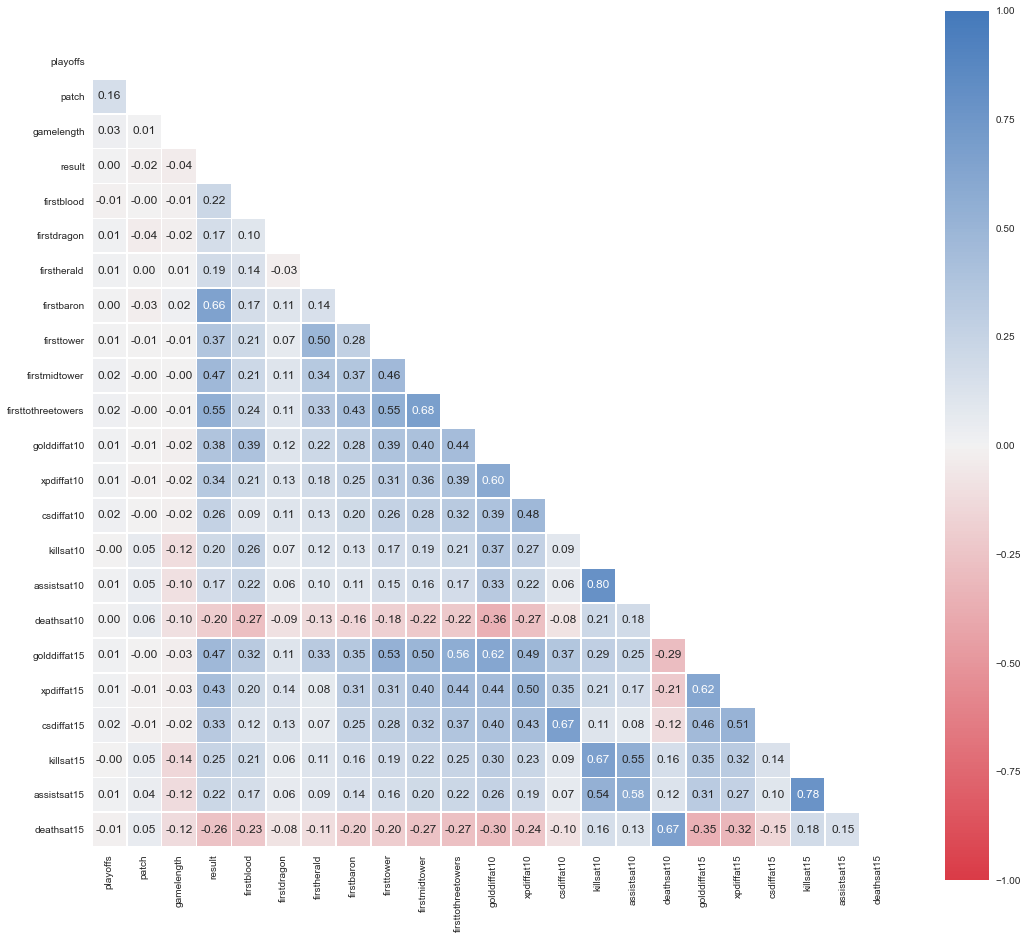
\includegraphics[width=1\textwidth]{figures/CorrMat1}
    \caption{A matrix of correlations between features in the dataset}
    \label{fig:CorrMat1}
\end{figure}

\begin{figure}[h!]
    \centering
    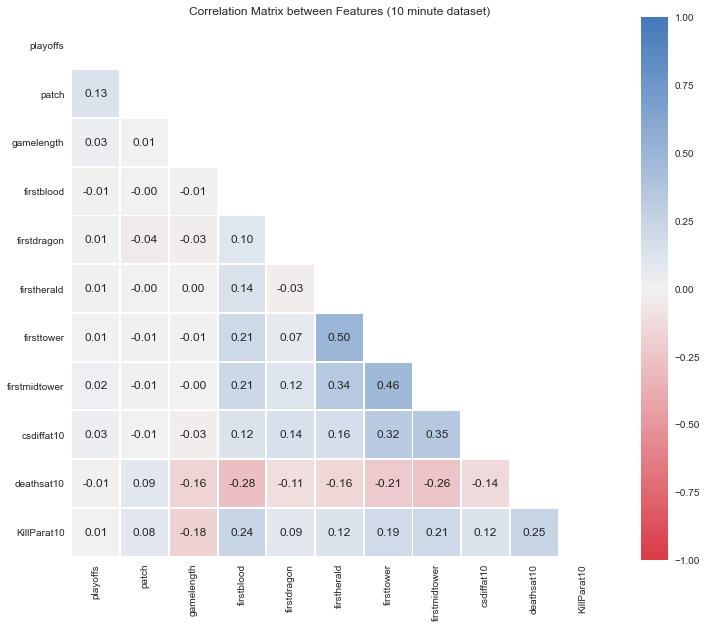
\includegraphics[width=1\textwidth]{figures/CorrMat10}
    \caption{A matrix of correlations from the 10-minute dataset}
    \label{fig:CorrMat10}
\end{figure}

\begin{figure}[h!]
    \centering
    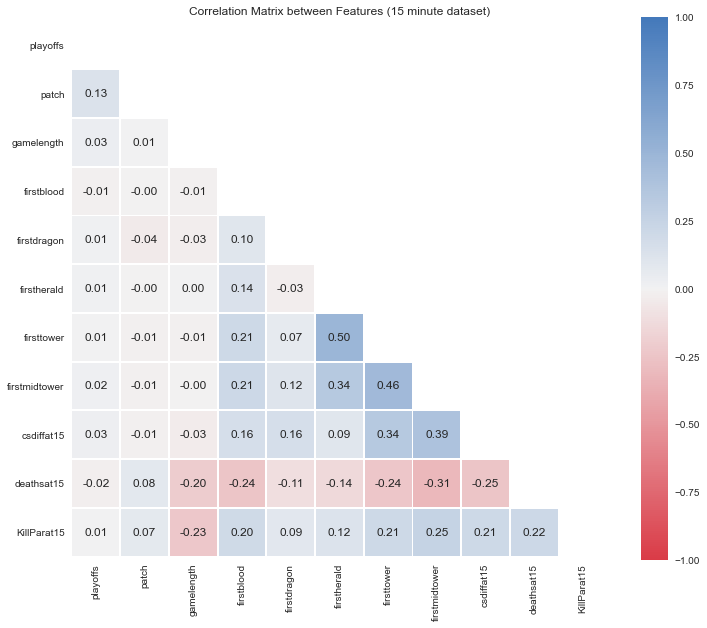
\includegraphics[width=1\textwidth]{figures/CorrMat15}
    \caption{A matrix of correlations from the 15-minute dataset}
    \label{fig:CorrMat15}
\end{figure}

\begin{figure}[h!]
    \centering
    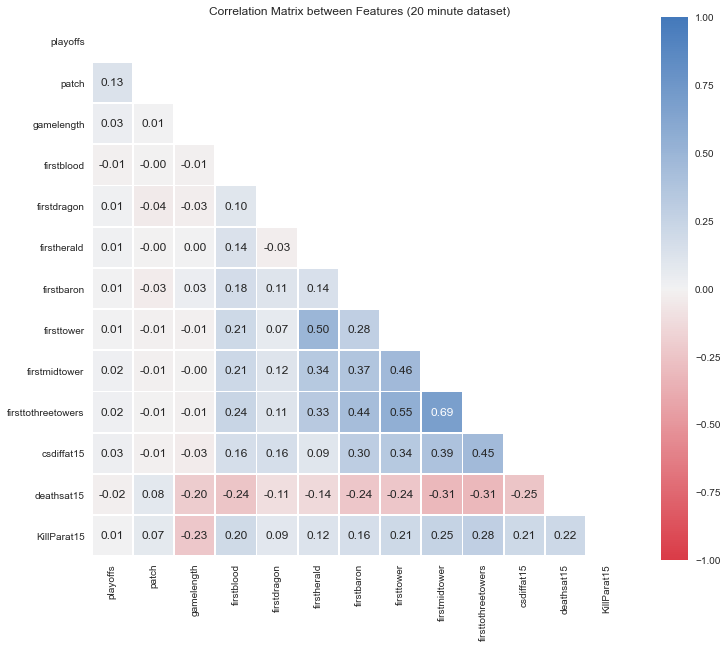
\includegraphics[width=1\textwidth]{figures/CorrMat20}
    \caption{A matrix of correlations from the 20-minute dataset}
    \label{fig:CorrMat20}
\end{figure}